\documentclass[11pt]{book}              % Book class in 11 points
\usepackage[utf8x]{inputenc} 
\usepackage[italian]{babel} 
\parindent0pt  \parskip10pt             % make block paragraphs
\raggedright                            % do not right justify

\usepackage{amsmath}
\usepackage{graphicx}
%\usepackage{fancyhdr}



\usepackage{fancyhdr}
\pagestyle{fancy}
\evensidemargin=1cm 
\oddsidemargin=1cm


%\usepackage[latin1]{inputenc}

\usepackage{graphicx}
\usepackage{hyperref}
\hypersetup{
    colorlinks,
    citecolor=black,
    filecolor=black,
    linkcolor=black,
    urlcolor=black
}
\cfoot{}
\rfoot{\thepage\ di 16}
\renewcommand{\footrulewidth}{0.4pt}
\newcommand{\numref}[1]{\textsl{\nameref{#1} (\ref{#1})}}

\renewcommand{\chaptermark}[1]{%
\markboth{\thechapter.\ #1}{}}

\renewcommand{\sectionmark}[1]{\markright{\thesection.\ #1}}


\begin{document}
\frontmatter

\begin{titlepage}
\centering  
\textbf{\huge{Università degli Studi di Padova}} \\
\vspace{0.3cm}
\huge{Dipartimento di Matematica} \\
\vspace{0.3cm}
\LARGE{Corso di Laurea in Informatica} \\

\vspace{1cm}

\includegraphics[scale=0.2]{img/Logo_Unipd.png}  \\
\vspace{1cm}
\hspace{0.5cm}\textbf{\LARGE{ Sviluppo di dispositivo embedded per la gestione di un pluviometro con Arduino}}\\
\vspace{0.5cm}
\textit{Relazione Finale laurea triennale}\\
\vspace{0.5cm}

\begin{flushleft}
\textit{Relatore} \hfill \textit{Laureando}\\
Prof. Tullio Vardanega \hfill Marco Gregorini

\end{flushleft}
\line(1, 0){360}\\
\textsc{\small{Anno accademico 2015 - 2016}}
\end{titlepage}


\newpage
\thispagestyle{empty}
\vspace*{\fill}

Marco Gregorini: \textit{Sviluppo di dispositivo embedded per la gestione di un pluviometro con Arduino,} Relazione Finale laurea triennale, \copyright Feb 2015

\newpage




\chapter{Sommario}

\section{Premessa}


Il seguente documento ha lo scopo di illustrare il lavoro svolto durante l'attività di stage dallo laureando Gregorini Marco, presso la sede del servizio informatico e di reti dell'agenzia regionale ARPAV, a Padova. Lo studente intende descrivere in modo critico e oggettivo le attività svolte durante il suo percorso di lavoro, della durata di circa trecentoventi ore, e i riscontri avuti con questa esperienza.

\section{Contenuti}

Nel documento vengono descritte le attività svolte per il completamento del progetto proposto da ARPAV, le necessità che hanno creato l'opportunità di lavoro per uno studente laureando e le prospettive che il progetto apre per il futuro.
I contenuti vengono esposti in quattro capitoli:

\begin{enumerate}
	\item \textbf{\nameref{1.0}:} descrizione generale dell'azienda. Dall'organizzazione interna agli obbiettivi che si pone;
	\item \textbf{\nameref{2.0}:} lo stage visto dal punto di vista dell'ente. Dai motivi che hanno evidenziato una necessità di uno stage, alla presentazione del progetto;
	\item \textbf{\nameref{3.0}:} lo stage visto dal punto di vista dello studente. Dalla pianificazione alla realizzazione;
	\item \textbf{\nameref{4.0}:} analisi retrospettiva dell'esperienza fatta. Valutazione critica dei risultati ottenuti, descrizione delle capacità e abilità acquisite, valutazione dello svolgimento del lavoro svolto.
\end{enumerate}

I termini che necessitano di spiegazione verranno descritti nel glossario e identificati alla loro prima occorrenza così\ped{g} .
\newpage
\thispagestyle{empty}

\tableofcontents    

\newpage
\thispagestyle{empty}

                  
\mainmatter       
  


\chapter{Profilo dell'Agenzia}
\label{1.0}
\thispagestyle{fancy} 

ARPAV\ped{g} è l'agenzia regionale per la prevenzione e protezione ambientale del Veneto, operativa dal 3 Ottobre 1997 in seguito alla Legge Regionale n32° del 18 Ottobre 1996.

\begin{figure}[htbp]
	\centering
	
\includegraphics[scale=0.7]{./capitoli/capitolo1/img/logoARPAV.jpg}
	\caption{logo dell'agenzia}
\end{figure}

Le attività competenti riguardano la tutela, il controllo, il recupero dell'ambiente e per la prevenzione e promozione della salute collettiva al fine di conseguire la massima efficacia nell'individuazione e nella rimozione dei fattori di rischio per l'uomo e per l'ambiente. Le funzioni principale dell'agenzia riguardano attività tecnico-scientifiche per il monitoraggio, tutela e prevenzione di acqua, aria (inquinamento acustico ed elettromagnetico negli ambienti di vita), suolo, rifiuti solidi e liquidi, radioattività ambientale ed infine ai rischi di incidenti rilevanti attività industriali. L'esercizio delle attività di monitoraggio e prevenzione vengono effettuate in coordinazione con le unità locali socio sanitarie.\\
L'agenzia è suddivisa in vari organi operativi, i quali hanno funzionalità specifiche a seconda del ruolo che ricoprono. La suddivisione degli incarichi e delle competenze e la corretta comunicazione fra i vari dipartimenti, permette di gestire questo vasto ente in modo efficiente e sistematico.\\
Lo \textit{stage} in oggetto è stato svolto presso il servizio informatico e di reti. In questa sede vengono svolte le mansioni per la gestione dell'infrastruttura informatica e delle risorse strumentali hardware di tutta l'agenzia e attività di ricerca e sviluppo inerenti.

\begin{table}[htbp]
\centering
\begin{tabular}{|p{0.95\textwidth}|}
\hline

\begin{itemize}

    \item gestione e coordinamento delle banche dati dell'agenzia;
	
	\item assistenza sulle applicazioni informatiche dell'agenzia;
	
	\item definizione degli indicatori ambientali e dei rapporti;
	
	\item fornitura degli standard operativi, architetture delle realizzazioni, attivazione e gestione tecnica dei portali internet/intranet;
	
	\item gestione connettività aziendale, voce dati;
	
	\item gestione tecnico operativa per il funzionamento, la manutenzione e la connettività delle reti di monitoraggio dell'azienda.
\end{itemize}
	\\
	
\hline
\end{tabular}
\caption{mansioni dipartimento Servizio Informatico e Reti}
\end{table}

\section{Cosa offre: Prodotti e Servizi}

In questa sezione vengono elencati e descritti le tipologie di prodotti che ARPAV produce e i tipi diversi di servizi che offre, ponendo particolare attenzione a ciò che viene erogato dalla sede dello \textit{stage}.

\subsection{I Prodotti di ARPAV}

Non essendo un'azienda a scopo di lucro, ma un'agenzia regionale, ARPAV è tenuta alla parità di bilancio. L'orientamento generale non è propenso alla distribuzione e vendita di prodotti quindi, ARPAV, per lo più, collabora con altre aziende o enti per realizzare progetti in ambito ambientale come \textit{patner, subcontractor\ped{g}} o \textit{leader}.



\begin{longtable}{ p{0.2\textwidth} | p{0.3\textwidth} | p{0.5\textwidth}}

\textbf{Logo}& \textbf{Ruolo \& Nome}&  \textbf{Descrizione}\\

 \endhead
\midrule
\vfill 
\includegraphics[scale=0.8]{./capitoli/capitolo1/img/alpini} & \vfill \textbf{{\color{Plum}Ruolo}: \textit{Patner}} \newline \vfill \textbf{{\color{ForestGreen}SedAlp}: Programma Spazio Alpino}  &
 Sviluppo e \textit{testing} di politiche e strumenti utili alla gestione integrata del trasporto di sedimenti nei bacini alpini al fine di ridurre il rischio legato al trasporto solido e allo stesso tempo di migliorare la condizione ecologica degli ambienti acquatici e ripararli e ridurre l'impatto ambientale creato dalle centrali idroelettriche. \textit{\href{http://www.alpine-space.eu/}{website}}\\
\midrule
\vfill 
\includegraphics[scale=0.7]{./capitoli/capitolo1/img/med} & \vfill \textbf{{\color{Plum}Ruolo}: \textit{Leader}} \newline \vfill \textbf{{\color{ForestGreen}CAIMANs}: Programma Med}  & Valutando l'impatto sulla qualità dell'aria da parte delle navi crociera e in generale delle navi passeggeri, il progetto mira a porre le basi per l'identificazione dei punti critici e per proporre orientamenti per futuri progetti e politiche trasnazionali che affrontino la mitigazione dell'inquinamento atmosferico dovuto al traffico navale passeggeri. \textit{\href{http://www.medmaritimeprojects.eu/section/caimans}{website}} \\
\midrule
\vfill 
\includegraphics[scale=0.7]{./capitoli/capitolo1/img/park} & \vfill \textbf{{\color{Plum}Ruolo}: \textit{Patner}} \newline \vfill \textbf{ {\color{ForestGreen}GuardEn}: Programma South East Europe } & Sviluppo e \textit{testing} di un possibile quadro di riferimento finalizzato al supporto di un programma di implementazione di locali strategie per la gestione e prevenzione del rischio ambientale legato all'attività agricola e agroalimentare. In particolare per i territori interessati dall'inquinamento del suolo e dell'acqua, da proporre per l'applicazione alle aziende del settore. \textit{\href{http://www.southeast-europe.net/en/}{website}}\\
\midrule
\vfill 
\includegraphics[scale=0.7]{./capitoli/capitolo1/img/interr} & \vfill \textbf{{\color{Plum}Ruolo}: \textit{Patner}} \newline \vfill \textbf{{\color{ForestGreen}3PClim}: Programma Interreg IV Italia – Austria} &   Aggiornamento della climatologia delle Alpi orientali, con la produzioni di cartografie tematiche, elaborazioni e proiezioni climatiche. \textit{\href{http://www.interreg.net/it/programma/programma.asp}{website}}\\
\midrule
\vfill 
\includegraphics[scale=0.7]{./capitoli/capitolo1/img/resmia} & \vfill \textbf{{\color{Plum}Ruolo}: \textit{Patner}} \newline \vfill \textbf{{\color{ForestGreen}RE.S.M.I.A.}: Programma POR – FESR Veneto} & Progetto pilota di ricerca industriale con l’obiettivo di potenziare ed integrare la rete di monitoraggio ambientale a disposizione di ARPAV. \textit{\href{http://www.resmia.eu/}{website}} \\
\bottomrule
\caption{progetti ARPAV}
\end{longtable}

Il dipartimento di informatica e reti, in collaborazione con CIVEN\ped{g}, durante il periodo stagistico stava seguendo con particolare attenzione \textbf{RE.S.M.I.A.}\ped{g}. Il progetto consiste nel potenziamento dell'infrastruttura delle stazioni di monitoraggio ambientale attualmente a disposizione di ARPAV, con la progettazione ed installazione di sensori. Il nuovo concetto di stazione farà uso di tecnologia WSN\ped{g}, applicativi \textit{Web-Based}\ped{g} e sarà caratterizzato dall'ottimizzazione della efficienza energetica del sistema. \\


Le finalità principali del progetto sono:
\begin{itemize}

	\item \textbf{minimizzazione dell'impatto ambientale dall'installazione delle stazioni di monitoraggio:} utilizzo di tecnologie per l'auto-alimentazione dell'impianto e utilizzo di tecnologie \textit{wireless} per ridurre al minimo l'invasione ambientale e con sperimentazione di nuovi sensori elettrochimici nanostrutturati per il monitoraggio in sito di metalli pesanti;
	\item \textbf{riduzione dei costi di produzioni ed installazione:} utilizzo di nuovi \textit{hardware} a basso costo con ottime prestazioni, bassa necessità di manutenzione e semplice installazione, anche in presenza di condizioni morfologiche del territorio estremamente critiche. Realizzazione di prodotti in grado di essere installati da qualunque persona, in particolare volontari sprovvisti di preparazione;
	\item \textbf{tutela dell'ambiente:} monitoraggio delle matrici ambientali anticipando anche le disposizioni legislative e ponendo attenzione alle tematiche sentite dall'opinione pubblica in tema di salute, quale ad esempio il monitoraggio di nanoparticelle in aria;
	\item \textbf{prevenzione dei rischi:} determinazione delle soglie minime di allarme dei parametri ambientali reperibili in tempi brevi per l'intero territorio della Regione del Veneto;

\end{itemize}

\begin{figure}[htbp]
\centering
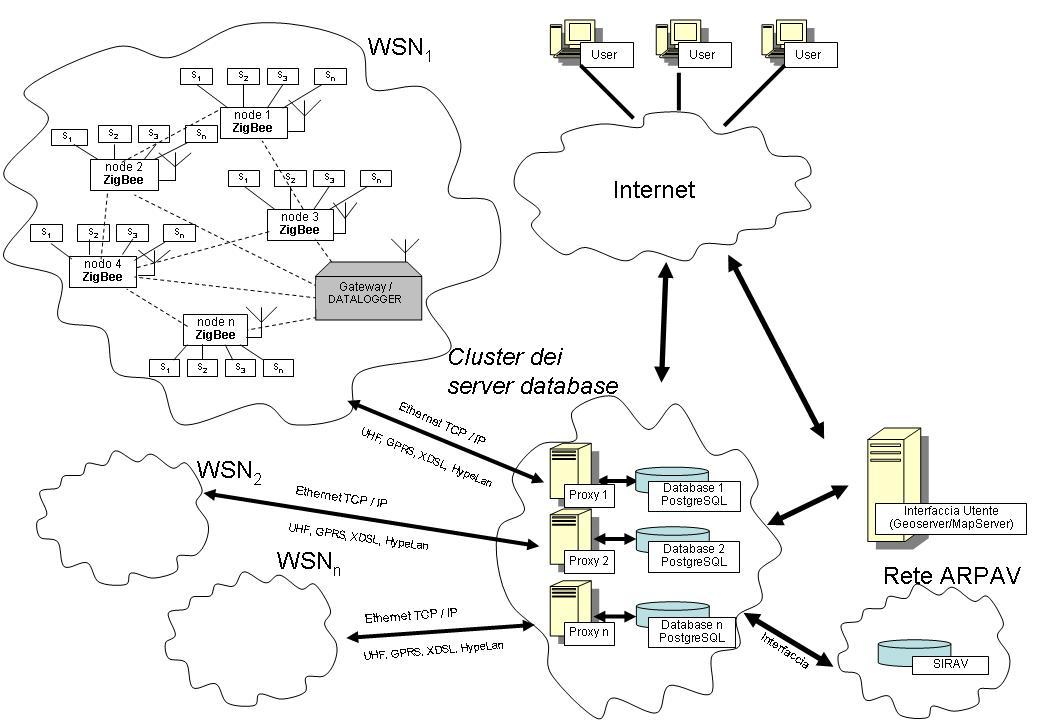
\includegraphics[scale=0.3]{./capitoli/capitolo1/img/retiresmia}
\caption{schema reti RESMIA}
\end{figure}

Il dipartimento di informatica e reti ha il compito di incrementare la struttura del sistema di salvataggio dei dati e di potenziare l'interfaccia \textit{web} che rappresenta graficamente su un'opportuna mappa la dislocazione dei sensori e ed effettuare opportune interrogazioni sui dati forniti tramite \textit{Map Server}\ped{g}.

\subsection{I Servizi di ARPAV}

L'agenzia regionale offre una vasta gamma di servizi, i quali possono essere suddivisi in due macro categorie: servizi ambientali e servizi online. I primi, offrono un servizio su richiesta o erogati da ARPAV, i secondi invece sono servizi passivi offerti dal portale \textit{internet}, i cui fruitori possono accedervi tramite \textit{network}.  \textit{\href{http://www.arpa.veneto.it/servizi-ambientali}{website}}

\subsubsection{Servizi Ambientali}

\begin{longtable}{ p{0.3\textwidth} | p{0.3\textwidth} | p{0.4\textwidth}}
\textbf{Nome}& \textbf{Possibili Fruitori}&  \textbf{Descrizione} \\
\endhead

	\midrule
	\textbf{{\color{OliveGreen}Acquisti pubblici verdi-GPP\ped{g}}} & Pubbliche amministrazioni locali o nazionali  & Informazione delle pubbliche amministrazioni circa l'adozione di pratiche d'acquisto verdi che riducono l'uso di risorse naturali, la produzione di rifiuti, i rischi ambientali \\
	\midrule
	\textbf{{\color{OliveGreen}Certificazioni ambientali}} & Imprese soprattutto piccole e medie &  Diffusione all'interno del mondo produttivo di una nuova cultura di sistema per la gestione consapevole ed ecocompatibile dell'ambiente attraverso lo sviluppo di progetti, strumenti, protocolli ad hoc\\
	\midrule
	\textbf{{\color{OliveGreen}Comunicazione}} & Cittadini & Promozione delle attività di educazione ed informazione ambientale dei cittadini \\
	\midrule
	\textbf{{\color{OliveGreen}Progetti \& Cooperazione}} & Aziende, imprese, enti pubblici o regioni & Avvio e realizzazione di progetti, avvio di relazioni internazionali generalmente finanziati da fondi dell'Unione Europea \\
	\midrule
	\textbf{{\color{OliveGreen} Grandi opere}} & Aziende coinvolte in appalti pubblici in Veneto & attività di audit preventivo e di monitoraggio ambientale per garantire la compatibilità ambientale, il corretto inserimento dal punto di vista urbanistico, ambientale, trasportistico e sociale delle Grandi Opere \\
	\midrule
	\textbf{{\color{OliveGreen} Educazione per la sostenibilità}} & Chiunque &  Attività di educazione, informazione e comunicazione ambientale, protezione della natura al fine di promuovere e sviluppare comportamenti sostenibili \\
	\midrule
	\textbf{{\color{OliveGreen} IPPC\ped{g} e  Servizi alle aziende}} & Aziende ed Imprese & Consulenze sul piano di monitoraggio e controllo in fase istruttoria per il rilascio dell'autorizzazione integrata ambientale, ispezioni integrate ambientali nelle aziende IPPC del Veneto\\
	\midrule
	\textbf{{\color{OliveGreen} Pronta disponibilità}} &  Dipartimenti di Prevenzione delle ULSS regionali Organi di polizia giudiziaria &  Attività di analisi immediata di aria, acqua e suolo secondo le modalità previste\\
	\midrule
	\textbf{{\color{OliveGreen} Rischio industriale}} & Industrie & Individuazione, classificazione e probabilità dei pericoli provenienti dalle industrie che utilizzano o detengono sostanze chimiche per le loro attività \\
	\midrule
	\textbf{{\color{OliveGreen} Sicurezza impiantistica}} & Comuni, ASL, Prefettura, Procura & Verifica della corretta funzionalità di impianti e macchinari installati in ambienti di lavoro o di vita e soggetti a controlli periodici \\
	\bottomrule
	

\caption{servizi ambientali ARPAV}
\end{longtable}

\subsubsection{Servizi Online}

\begin{longtable}{p{0.3\textwidth}|p{0.7\textwidth}}
\textbf{Nome} & \textbf{Descrizione} \\
\endhead

\midrule
\textbf{{\color{Plum} Accesso informazioni ambientali}} & Accesso del pubblico all'informazione ambientale detenuta o prodotta da soggetti pubblici avviene anche mediante l'utilizzo delle tecnologie informatiche e dei mezzi di telecomunicazione \\
\midrule
\textbf{{\color{Plum} Glossari Ambientali}} & Strumento di informazione aggiornata ed esaustiva che ARPAV mette a disposizione dei cittadini per favorire la comprensione di termini 'ambientali' maggiormente utilizzati \\
\midrule
\textbf{{\color{Plum} Iscrizione bollettini}} & Iscrizione alla mailing list consente di ricevere i bollettini Meteo direttamente nella propria casella di posta elettronica. Meteo Veneto, Dolomiti Meteo, Meteo Spiagge e Meteo Garda i bollettini per cui è disponibile il servizio \\
\midrule
\textbf{{\color{Plum} Iscrizione bollettini via sms}} & Sottoscrivendo un abbonamento è possibile ricevere via sms i contenuti di alcuni bollettini prodotti per l'area delle Dolomiti. Dolomiti meteo e Dolomiti Neve e Valanghe i bollettini per i quali è disponibile il servizio \\
\midrule
\textbf{{\color{Plum} Iscrizione \textit{newsletter}}} &  E' possibile ricevere periodicamente nella propria casella di posta le \textit{newsletter} con informazioni su eventi, contenuti e attività \\
\midrule
\textbf{{\color{Plum} Iscrizione applicativo web ORSO }} &  Programma per il monitoraggio del flusso dei rifiuti attraverso le Regioni d'Italia, con standard di riferimento comuni che garantiscano rappresentatività delle informazioni raccolte, oltre ad agevolare lo scambio di informazioni finalizzato alla corretta gestione dei rifiuti per i Comuni e gestori degli impianti \\
\midrule
\textbf{{\color{Plum} Iscrizione a IRRIFRAME}} & Servizio che permette alle aziende registrate di salvare il proprio profilo colturale e di personalizzare l'informazione irrigua fornita dal servizio comunicando in tempo reale dati locali \\
\midrule
\textbf{{\color{Plum} Link utili}} & Una rassegna di 'siti utili'; la suddivisione per argomenti e temi permette di individuare facilmente i riferimenti cercati \\
\midrule
\textbf{{\color{Plum} Richiesta pubblicazioni}} & Possibilità di richiedere una copia delle pubblicazioni edite da ARPAV attraverso posta elettronica e la compilazione di un modulo \\
\bottomrule

\caption{servizi online di ARPAV}
\end{longtable}

\newpage

\section{Organizzazione Interna}

ARPAV è un'agenzia regionale che lavora per il completamento di progetti a livello regionale, nazionale ed internazionale ed offre tutta una serie di servizi a livello regionale e non. Per fare ciò necessita di una  organizzazione interna ben strutturata, suddivisa in vari organi operativi, ognuno dei quali ricopre una funzionalità specifica e si interfaccia con un altra secondo protocolli prestabiliti. ARPAV è dotata di una autonomia interna negli ambiti amministrativi, organizzativi e tecnico contabile e di diverse figure professionali che garantiscono un approccio multidisciplinari.

\begin{figure}[htbp]
\centering
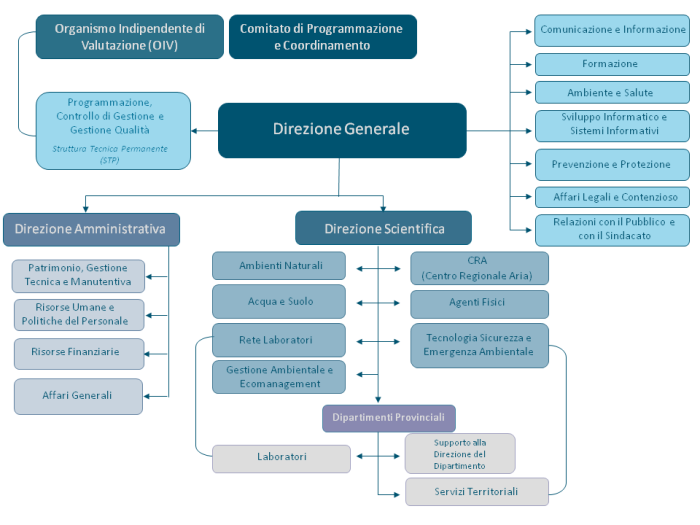
\includegraphics[scale=0.7]{./capitoli/capitolo1/img/organigramma}

\caption{organigramma struttura ARPAV}

\end{figure}

A livello macroscopico è composta da una \textbf{Direzione Generale}, che a sua volta si ramifica in più aree funzionali di natura amministrativa e tecnico-scientifica, due \textbf{Dipartimenti regionali} e sette \textbf{Dipartimenti provinciali}. I dipartimenti regionali e provinciali per la realizzazione dei programmi ed attività di competenza godono di una autonomia gestionale nei limiti delle risorse loro assegnate dalla direzione generale.\\
La sede dello stage si trova all'interno dell'area della \textbf{direzione amministrativa}, in particolare nel sottoinsieme della \textbf{gestione tecnica}.\\
L'organizzazione interna al dipartimento di informatica è riassumibile così:

\begin{figure}[htbp]
	\centering
	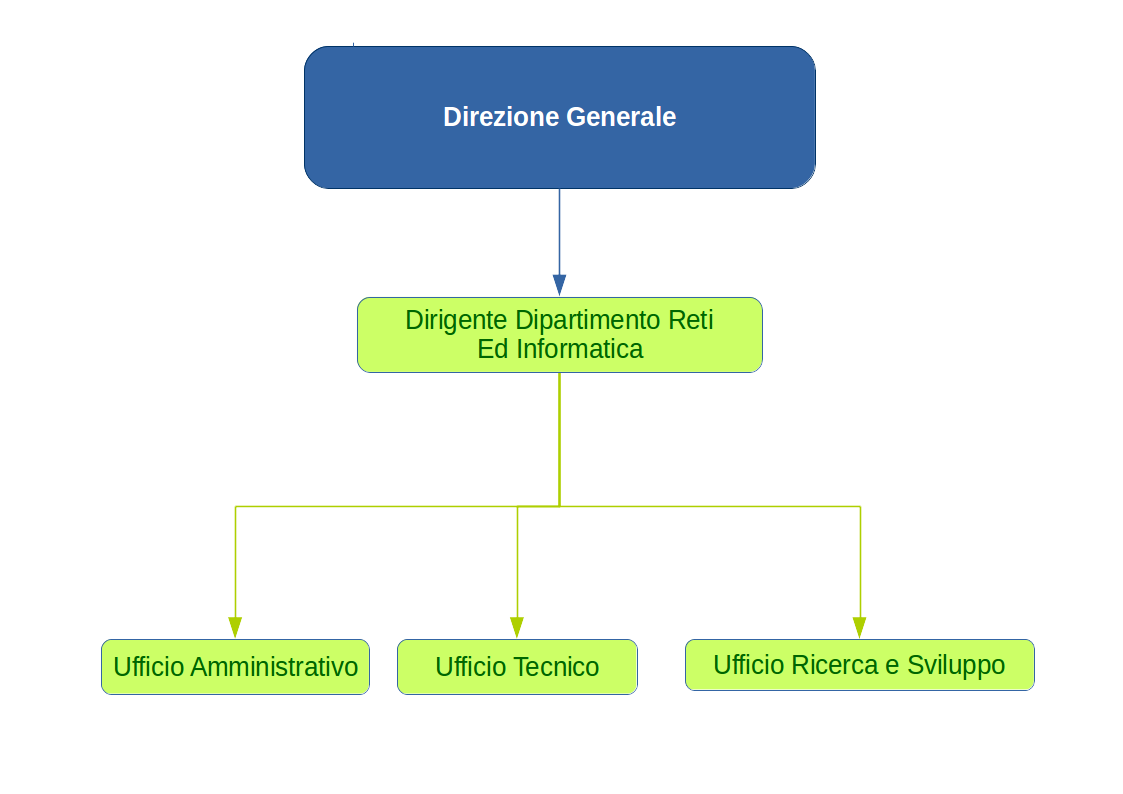
\includegraphics[scale=0.4]{./capitoli/capitolo1/img/organigrammaDip}
	\caption{organigramma Dipartimento Informatica e Reti}
\end{figure}

\begin{itemize}

	\item \textbf{Direttore:} figura a cui tutti fanno riferimento, ha il compito di relazionarsi con le aziende esterne per accordare collaborazioni nei progetti assegnati dalla \textbf{Direzione Generale}. Deve anche approvare i bilanci economici e gestire le risorse umane;
	\item \textbf{Ufficio Amministrativo:} ufficio con il compito di adempiere alle funzioni amministrative del dipartimento;
	\item \textbf{Ufficio di Ricerca e Sviluppo:} ufficio esecutivo in cui si sviluppano o si fa manutenzione sui progetti;
	\item \textbf{Ufficio Tecnico:} ufficio composto da tecnici addetti alla manutenzione del sistema di reti dell'intero ente.
	
\end{itemize}
\subsection{Processi di Sviluppo}


I processi di sviluppo all'interno di  ARPAV non possono essere facilmente standardizzati, in quanto ogni settore operativo ha necessità di agire in modo differente rispetto gli altri. E' dunque previsto che ogni dipartimento organizzi i propri processi in base alla propria funzione, restando conforme alle linee guida dettate dalla \textbf{Direzione Centrale} tramite documenti specifici: 

\begin{itemize}
	\item \textbf{\textit{Piano Triennale Regionale di Educazione Ambientale}}\ped{g}: documento di validità triennale in cui si definiscono le linee guida dell'agenzia, gli obiettivi da raggiungere e me metodologie di crescita;
	\item \textbf{\textit{Documento di Programmazione per l'Informazione, la Formazione e l'Educazione Ambientale (IN.F.E.A.)}}\ped{g}: documento in cui vengono definiti provvedimenti, progetti (di durata pluriennale) e azioni che mirano all'adempimento degli obiettivi prefissati dal Piano Triennale di Educazione Ambientale;
	\item \textbf{\textit{Programma Triennale per la Trasparenza e Integrità}}: documento di validità triennale, aggiornato annualmente, in cui vengono definiti i processi per garantire un livello di trasparenza, legalità e sviluppo della coltura dell'integrità.
	
	
\end{itemize}

\begin{figure}[htpb]
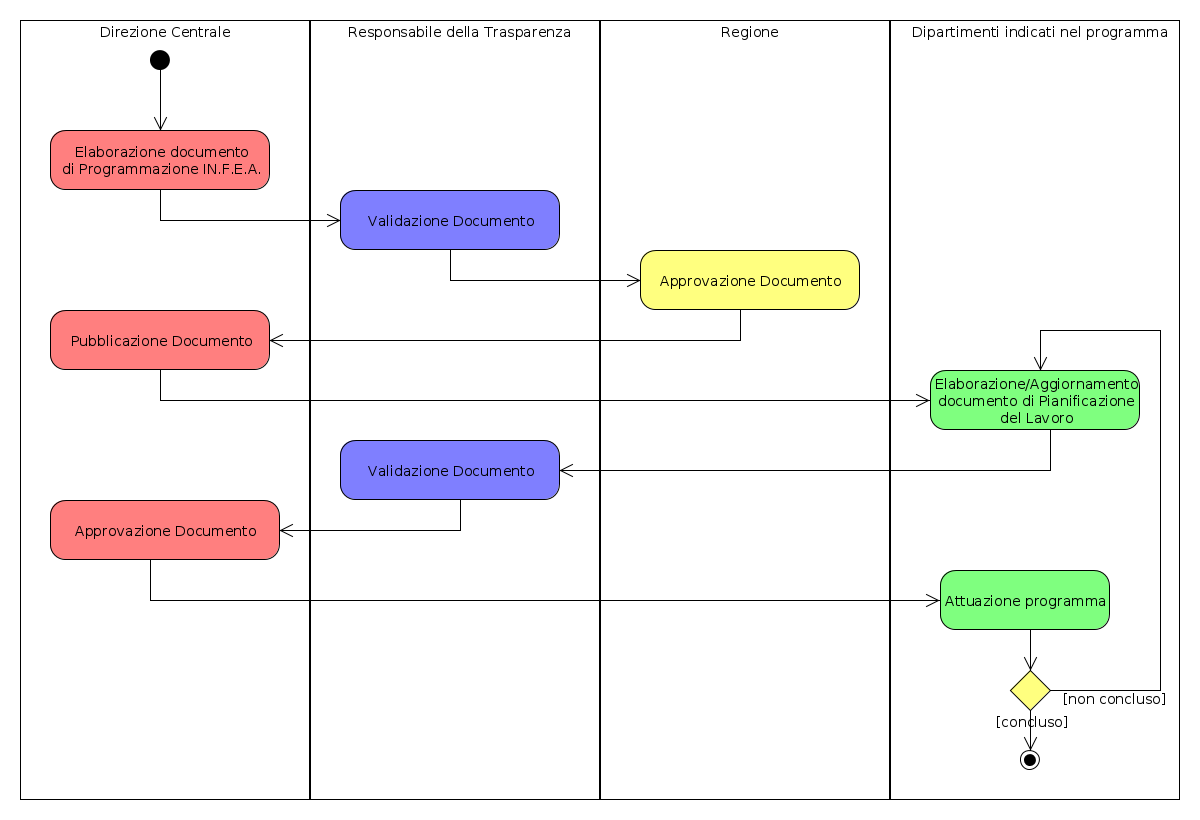
\includegraphics[scale=0.33]{./capitoli/capitolo1/img/attivita_programma}
\caption{diagramma attività approvazione progetti}
\end{figure}

Nel documento di Programmazione IN.F.E.A. vengono definite le finalità che i progetti triennali intendono perseguire. E' compito dei dipartimenti, a cui è stata delegata la realizzazione del progetto, dichiarare la gestione del \textit{budget}, gli interventi di aziende private esterne e la pianificazione degli obiettivi intermedi. I dipartimenti sono dunque tenuti a realizzare un documento di \textit{Pianificazione del Lavoro}, nel quale verranno descritte le \textit{milestone} che si intendono raggiungere alla fine di ogni anno e, in particolare, la suddivisione del lavoro su base annuale. Il documento viene quindi aggiornato in tre occasioni:

\begin{itemize}
	\item Inizio anno: vengono definiti i traguardi che si realizzeranno durante l'anno in corso, le ore preventivate per attività e il \textit{budget} che si presume di spendere;
	\item Dopo sei mesi: viene aggiornato lo stato di avanzamento del progetto con relative modifiche;
	\item Fine anno: viene aggiornato lo stato di avanzamento del progetto con relative modifiche del piano di lavoro triennale e ci si predispone la stesura del successivo anno di lavoro.
\end{itemize}

Ogni incremento del documento viene visionato dal responsabile della trasparenza e approvato dalla Direzione Centrale.\\



In particolare, nel dipartimento sede dello \textit{stage}, dovendo lavorare su progetti informatici ampi e complessi, l'approccio utilizzato è di tipo \textit{top-down}. Progetti che coinvolgono l'impiego di risorse per periodi duraturi, richiedono una accurata e solida conoscenza delle problematiche che si devono affrontare e, in particolare, una solida ed accurata progettazione. Tramite l'approccio \textit{top-down} è possibile spezzare un problema iniziale complesso in più sottoproblemi, la cui realizzazione risulta più efficacemente semplice.\\




\begin{figure}[htpb]
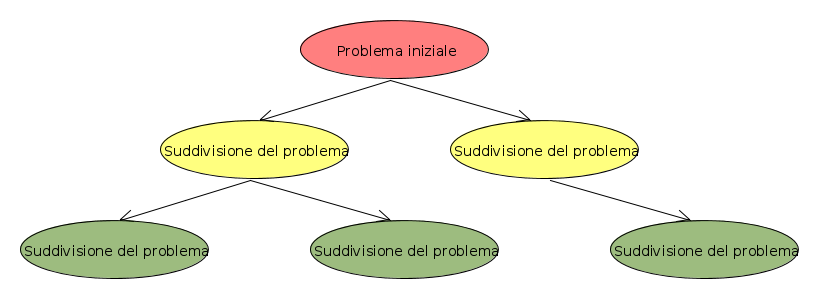
\includegraphics[scale=0.4]{./capitoli/capitolo1/img/probo}
\caption{raffigurazione divisione problema approccio top-down}
\end{figure}


 
\subsection{Metodologie di Supporto ai Processi}


L'attitudine a svolgere progetti su piani pluriennali non mi ha reso semplice comprendere la tipologia di processo attuato all'interno della sede dello \textit{stage}. Durante la mia partecipazione come stagista, ho capito che vengono sistematicamente svolte attività di \textit{Analisi dei Requisiti}, \textit{Progettazione}, \textit{Test e Rilascio} e \textit{Manutenzione}. 
\begin{figure}[htbp]
	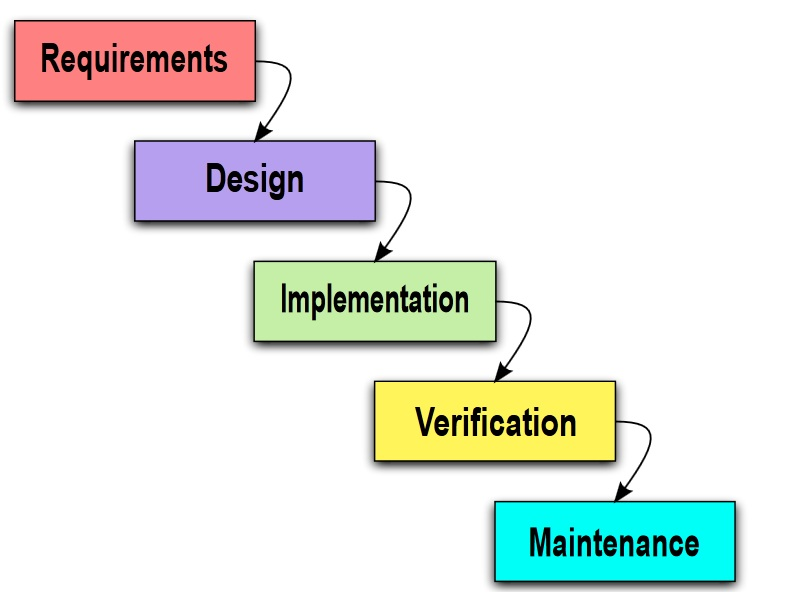
\includegraphics[scale=0.3]{./capitoli/capitolo1/img/cascata}
	\caption{ciclo di vita a cascata}

\end{figure}

Lavorare a progetti che prevedono una durata di sviluppo su base annuale, richiedono una ottima identificazione dei problemi, progettazione di partenza. L'utilizzo di documentazione risulta essenziale, poiché è probabile che subentrino nuove persone all'interno del progetto.
Ne ho dedotto dunque che il ciclo di vita assunto dal dipartimento di informatica è un modello a cascata.


\subsection{Strumenti di Supporto ai Processi}

\subsubsection{Gestione Documenti}
La documentazione riguardante l'analisi dei requisiti viene raccolta all'interno dei server dedicati tramite il \textit{network} da loro gestito. Per altri documenti vengono molto utilizzati servizi come \textit{Google Drive}. 
 


\subsubsection{Ticketing}

Durante la mia presenza in sede ho potuto notare come gli strumenti di \textit{ticketing} fossero utilizzati in parte. Nonostante fossero presenti erano comunque necessarie riunioni per conoscere la situazione interna dei progetti.
\subsubsection{Gestione Calendario}

Per la gestione delle attività di gruppo, come riunioni ufficiali per il resoconto delle attività o la risoluzione di conflitti interni, viene utilizzato lo strumento \textit{Google Calendar}.




\section{Relazioni Esterne}


Essendo un'agenzia regionale finalizzata al monitoraggio e alla tutela dell'ambiente, ARPAV non ha un vero e proprio \textit{target} di clientela. \\
A seconda del ruolo che l'agenzia ricopre in un progetto (\textit{patner} o \textit{leader}) può collaborare con altre agenzie o aziende per fornire prodotti o migliorare infrastrutture. Altrimenti, attraverso i suoi servizi, può interfacciarsi con le singole imprese, industrie e  privati cittadini. 

\subsection{Orientamento all'Innovazione}
Gli obiettivi di ARPAV sono:
\begin{itemize}
	
\item    \textbf{la protezione}, attraverso i controlli ambientali che tutelano la salute della popolazione e la sicurezza del territorio;
\item \textbf{la prevenzione}, attraverso la ricerca, la formazione, l'informazione e l'educazione ambientale.
\end{itemize} 

L'innovazione nelle tecnologie, nei servizi e nelle infrastrutture portano ad un continuo raggiungimento dei due obiettivi preposti. ARPAV non ha come fine un guadagno, ma è un'agenzia regionale che è stata istituita per migliorare la qualità dell'ambiente che ci circonda e quindi la vita. Tramite processi di innovazione l'agenzia sarà in grado di: 
\begin{itemize}
	\item ridurre i costi dei propri servizi;
	\item diminuire i danni ambientali presenti;
	\item monitorare il territorio per la prevenzione dei rischi;
	\item fornire una rapida ed efficace risposta in caso di necessità.
	
\end{itemize}



\chapter{Lo Stage per ARPAV}
\label{2.0}
\thispagestyle{fancy} 

[:] introduzione del capitolo con la descrizione dei motivi per cui l'agenzia ricerca stagisti per affidare loro dei progetti da sviluppare.

\section{L'Esigenza di uno Stage}

[:] Sezione in cui descrivo i motivi per cui l'agenzia ha trovato la necessità di avviare questo specifico stage per questo progetto

\section{Presentazione del Progetto}

[:] Sezione in cui descrivo il progetto vero e proprio, in che cosa consiste e in quali realtà potrà essere inserito.

\subsection{Obbiettivo dello Stage}

[:] Sottosezione in descrivo gli obbiettivi che sono stati preposti all'inizio dello stage nel momento in cui ho preso visione dell'offerta fatta dall'agenzia.
La sezione inizia con una breve introduzione del piano di lavoro e la descrizione del significato di obbiettivo.

\subsubsection{Obbiettivi Minimi Richiesti}

[:] Elenco e descrizione degli obbiettivi minimi richiesti all'inizio dello stage.

\subsubsection{Obbiettivi Massimi Raggiungibili}

[:] Elenco e descrizione degli obbiettivi che l'agenzia desidera raggiungere, ma che non sono vincolanti alla conclusione dello stage.

\subsection{Finalità del Progetto}

[:] Sezione descrivo in dettaglio l'applicazione del prodotto dello stage nella realtà dell'ente e non.

\section{Vincoli di Progetto}

[:] Descrizione delle tipologie di vincoli che sono stati imposti nello stage.

\subsection{Vincoli di Dominio}

[:] Descrizione dei vincoli che dovranno essere soddisfatti dal progetto in termini di funzionalità, affidabilità e manutenibilità. 

\subsection{Vincoli Tecnologici}

[:] Descrizione dei vincoli riguardanti gli strumenti di lavoro, come framework e  e tecnologie obbligatori che dovranno essere utilizzati durante l'attività stagistica.

\subsection{Vincoli Metodologici}

[:] Descrizione dei vincoli metodologici che lo ho dovuto seguire durante tutta la fase dello stage.

\subsection{Vincoli Temporali}

[:] Descrizione dei vincoli temporali prefissati in base alle necessità dell'ente e i problemi di fattori esterni dovuti alla cooperazione di aziende terze per il completamento dello stage.


\chapter{L'Attività di Stage}
\thispagestyle{fancy} 

[:] Descrizione introduttiva del capitolo e delle sue sezioni

\section{Pianificazione del Lavoro}

[:] Sezione in cui descrivo la pianificazione a monte di tutta l'attività di stage in relazione con i vincoli precedentemente assunti assieme all'azienda.



\subsection{Preparazione al Lavoro di Stage}

[:] Sezione in cui descrivo come mi sono preparato per affrontare il lavoro dello stage il meno impreparato possibile, così da poter attutire possibili ritardi.

\subsubsection{Studio del Dominio}

[:] Sottosezione in cui spiego come mi sono affacciato al dominio richiesto per lo stage, assumendone tutti i pro, i contro, possibilità e criticità che ho riscontrato all'inizio dell'attività di stage.

\subsubsection{Studio delle Tecnologie}

[:] Sottosezione in cui descrivo, uno per uno, le tecnologie e gli strumenti necessarie per intraprendere lo stage e i supporti utilizzati per acquisire tali conoscenze.


\subsubsection{Criticità riscontrate}

[:] Descrizione delle possibili criticità riscontrate a fronte degli obbiettivi richiesti in relazione con il dominio e le mie conoscenze di base.



\section{Analisi dei Requisiti}
[:] Introduzione alla sezione e breve descrizione delle sottosezioni


\subsection{Classificazione dei Requisiti}

[:] Descrizione delle suddivisioni fatte per classificare i requisiti in modo tale da risultare chiari e comprensibili.


\subsection{Individuazione dei Requisiti}

[:] Descrizione dei metodi utilizzati per individuare i requisiti e visualizzazione degli stessi tramite tabella

\subsubsection{Strumenti Utilizzati}

[:] Elenco e descrizione degli strumenti utilizzati per il tracciamento dei requisiti

\subsection{Casi d'Uso}

[:] Descrizione del motivo per cui i casi d'uso non sono stati usati come mi ero prefissato ad inizio stage.

\subsection{Dettagli Degni di Nota}

[:] Sezione in cui prendo in considerazione alcuni requisiti particolari analizzandone gli aspetti di difficoltà, problematiche e metodi di risoluzione del problema.

\section{Progettazione e Codifica}

[:] Descrizione dell'attività di Progettazione e delle scelte fatte durante lo stage di incrementare la progettazione di volta in volta.

\subsection{Introduzione Architettura Hardware}

[:] Sezione in cui descrivo la composizione delle componenti hardware durante l'attività di progettazione e codifica e come poi queste si siano unificate in un unico componente successivamente durante i test.

\subsection{Introduzione Architettura Software}

[:] Descrivo brevemente l'architettura software nel suo complesso delle due componenti hardware.

\subsection{Architettura Libreria Scheda Master}

[:] Sezione in cui descrivo l'architettura della parte riguardante la libreria Master che permette di interfacciarsi con la Scheda Slave facilmente. 


\subsection{Architettura Scheda Slave}

[:] Sezione in cui descrivo l'architettura della Scheda Slave, che si interfaccia direttamente con il Pluviometro (questa parte è più ampia della precedente).

\subsection{Design Pattern Utilizzati}

[:] Sezione in cui elenco, motivo e descrivo i Design Pattern utilizzati nell'architettura del progetto.

\subsection{Dettagli Degni di Nota}

[:] Sezione in cui espongo alcuni dettagli rilevanti dell'architettura e soprattutto le difficoltà avute a causa delle limitate risorse hardware delle schede in mio possesso.

\subsection{Progettazione di Dettaglio e Codifica}

[:] Introduzione della sezione in cui spiego come mi sono adattato alle continue richieste di prototipi da parte dell'azienda e come ho organizzato la progettazione in modo da rendere il codice facilmente modificabile e riutilizzabile per una codifica incrementale.

\subsubsection{Dettagli Degni di Nota}

[:] Sezione in cui descrivo alcuni metodi della libreria Master che permettono un facile interfacciamento con la scheda Slave. In aggiunta come sia possibile aggiungere facilmente nuove funzionalità al sistema senza alcuna iterazione, ma incrementando il codice.

\subsection{L'Utilizzo dei Prototipi}

[:] Breve sezione in cui spiego come, a causa delle necessità aziendali, mi sia trovato costretto ad un continuo ciclo di "Progettazione, Codifica, Test, Progettazione Incrementale, Codifica, Test..", approccio diverso da quello affrontato durante il mio percorso accademico.

\section{Verifica e Validazione}

[:] Descrizione dell'attività di verifica e validazione e breve descrizione delle sottosezioni successive

\subsection{Analisi Statica}

[:] Elenco e descrizione degli strumenti utilizzati per l'analisi statica e alcuni valori che meritano d'esser presi in considerazione.

\subsection{Test sul Sistema Slave}

[:] Sezione in cui descrivo in dettagli i test effettuati sulla scheda Slave, in progressione con gli incrementi effettuati.

\subsection{Test sul Sistema Master Slave}

[:] Descrizione dei test effettuati sul sistema Slave integrato con le interazioni con la scheda master in progressione con gli incrementi effettuati.

\subsection{Test di Sistema}

[:] Descrizione dei test effettuati sull'intero sistema.

\subsection{Dettagli Degni di Nota}

[:] Descrizione del problema degli impulsi "falsi positivi" inviati dal pluviometro, riscontrati durante i test dell'intero sistema e soluzione.

\subsection{Consuntivo Orario Finale}

[:] Descrizione oggettiva e motivazione fra le discrepanze di orario preventivato ed effettivo in relazione agli obbiettivi raggiunti


\chapter{Valutazioni Finali}
\thispagestyle{fancy} 

\section{Raggiungimento degli Obbiettivi}

[:] Descrizione della sezione e introduzione delle sue sottosezioni

\subsection{Rendiconto degli Obbiettivi}

[:] Descrizione oggettiva fra obbiettivi soddisfati e non.


\section{Difficoltà Riscontrate}

[:] Elenco e descrizione delle difficoltà avute durante il lavoro di Stage con relativa soluzione attuata.

\section{Bilancio Formativo}

[:] Descrizione della sezione e introduzione delle sue sottosezioni.

\subsection{Preparazione Iniziale}

[:] Descrizione delle mie capacità iniziali e come queste mi siano state utili per il periodo di stage; corsi utili per la mia attività specifica e cosa invece mi è mancato.

\subsection{Esperienze Acquisite}

[:] Elenco e descrizione esperienze acquisite durante il periodo di stage suddivise fra competenze e conoscenze.

\subsection{Considerazioni Finali}

[:] Sezione in cui riassumo l'esperienza di stage facendone un'analisi obbiettiva. Considerando le mie capacità iniziali e relazionandole con l'offerta proposta dall'azienda, le difficoltà riscontrate e la mia preparazione e capacità di analizzare e affrontare i problemi riscontrati. Come mi siano stati più utili alcuni corsi universitari e come invece altri, se fatti in modo diverso, avrebbero potuto conferirmi maggior competenze per la riuscita dello stage. Ed infine cosa mi ha trasmesso lo stage in termini di competenze per l'inserimento nel mondo del lavoro.


\newpage





\end{document}